%% =====================================================================
%%  Revised manuscript -- IEEE Internet of Things Journal
%%
%%  Rewritten so that every claim matches the released implementation and
%%  the measured results in mdwgan/runs.  Author action items are marked
%%  with %% TODO.  Figures and tables are generated by
%%  mdwgan/analysis/figures.py and mdwgan/analysis/paper_tables.py.
%% =====================================================================
\documentclass[journal]{IEEEtran}

\usepackage{amsmath,amssymb,amsfonts}
\usepackage{algorithmic}
\usepackage{algorithm}
\usepackage{graphicx}
\usepackage{booktabs}
\usepackage{url}
\usepackage[hidelinks]{hyperref}

\graphicspath{{../paper_assets/}}

\begin{document}

\title{Resource-Aware Multi-Discriminator Wasserstein GAN Training\\
for the Internet of Vehicles}

\author{Farhoud~Jafari~Kaleibar,
        Amr~M.~Zaki,~\IEEEmembership{Member,~IEEE,}
        and~Marin~Litoiu,~\IEEEmembership{Senior~Member,~IEEE}
\thanks{The authors are with the Department of Electrical Engineering and
Computer Science, York University, Toronto, ON, Canada (e-mail:
farhoud@yorku.ca; mlitoiu@yorku.ca).}}

\markboth{IEEE Internet of Things Journal}%
{Jafari Kaleibar \MakeLowercase{\textit{et al.}}: Resource-Aware Multi-Discriminator WGAN Training for the IoV}

\maketitle

% =====================================================================
\begin{abstract}
Training generative models across vehicular edge nodes is constrained less by
final accuracy than by the cost of reaching it: vehicles hold a roadside unit's
coverage only briefly, and every synchronisation round consumes scarce
computation and spectrum. We present a resource-aware multi-discriminator
Wasserstein GAN framework for the Internet of Vehicles (IoV) in which roadside
units host conditional generators, vehicles act as critics over disjoint
trajectory partitions, and a game-theoretic step allocates training epochs
between the two sides from online estimates of their realised effectiveness and
per-epoch cost. We evaluate on real NGSIM trajectories against three federated
GAN baselines re-implemented under a common protocol, using proper scoring
rules rather than point error alone. The framework reaches a target accuracy
$2.2\times$ faster and with $2.4\times$ less computation than MD-GAN, while two
federated baselines do not reach it within the training budget; it also yields
by far the best-calibrated predictive distribution (PICP $0.75$ versus
$0.27$--$0.47$). Our ablation additionally reports two negative results that we
believe are useful to the community: a deep reinforcement-learning policy for
discriminator selection does not outperform a greedy single-line heuristic in
this setting, and the dominant factor in predictive quality is conditioning the
generator on observed trajectory context rather than any coordination
mechanism. All code, configurations and run records are released.
\end{abstract}

\begin{IEEEkeywords}
Internet of Vehicles, federated learning, generative adversarial networks,
resource-aware training, edge computing, trajectory prediction.
\end{IEEEkeywords}

% =====================================================================
\section{Introduction}
\IEEEPARstart{G}{enerative} models are increasingly used in vehicular networks
to synthesise trajectory data, augment rare safety-critical scenarios, and
support privacy-preserving data sharing \cite{devika2024vadgan,luo2025wgan}.
Training them across vehicular edge infrastructure, however, is a resource
orchestration problem rather than a modelling problem alone: which nodes should
participate, how a computation and communication budget should be divided among
them, and how service quality is sustained as connectivity changes with
mobility.

Prior work has largely reported this as an accuracy comparison. We argue that
in the vehicular setting accuracy at convergence is the wrong figure of merit.
A vehicle remains within a roadside unit's (RSU) coverage for a bounded time;
what matters operationally is how much accuracy is obtained per unit of
computation and spectrum consumed, and whether a usable model is reached before
the participants disperse. This paper is organised around that quantity.

We also take a deliberately conservative stance on evidence. Root mean square
error, the metric most commonly reported for this task, is minimised by
predicting the conditional mean --- precisely the mode collapse that adversarial
training is introduced to avoid. A generator that ignores its latent input
entirely scores well on it. We therefore report proper scoring rules (CRPS),
multi-modal error (minADE) and interval calibration (PICP) alongside RMSE, and
we subject every architectural claim to a paired significance test across seeds.

\textbf{Contributions.}
\begin{itemize}
\item A resource-aware multi-discriminator WGAN framework for IoV in which
      epoch allocation between generator and critics is set by a bounded
      best-response search whose effectiveness and cost parameters are
      re-estimated online from measured training behaviour
      (Section~\ref{sec:framework}).
\item An evaluation protocol for federated generative training in vehicular
      networks that reports cost-to-target and calibration rather than terminal
      point error, with three federated GAN baselines re-implemented under a
      common backbone, dataset partitioning and seed set
      (Section~\ref{sec:setup}).
\item A component ablation over $13$ variants and $5$ seeds, with paired
      significance tests, establishing which mechanisms are responsible for the
      observed behaviour --- including two negative results
      (Section~\ref{sec:results}).
\item Communication measurements obtained from an IEEE 802.11p simulation of the
      synchronisation round, reporting delivery ratio alongside latency
      (Section~\ref{sec:comm}).
\end{itemize}

%% TODO: if the MASCOTS paper [24] is cited as prior work of the authors,
%% state the delta explicitly here to avoid a self-plagiarism flag.

% =====================================================================
\section{Background and Related Work}
%% TODO: this section can be carried over from the submitted manuscript with
%% two changes: (i) HVS-GAN must be described as a server-coordinated federated
%% GAN with DDPG-based vehicle scheduling, which is what we re-implement in
%% Section V-C; (ii) add a paragraph on proper scoring rules motivating CRPS.

\subsection{Wasserstein GAN}
A GAN \cite{creswell2018gan} couples a generator that synthesises samples with a
discriminator that separates them from real data. The Wasserstein formulation
\cite{arjovsky2017wgan} replaces the Jensen--Shannon objective with the
Earth-Mover distance, which provides usable gradients even when the real and
generated distributions do not overlap. The critic is constrained to be
1-Lipschitz, enforced here by a gradient penalty. For consistency with the IoV
systems literature we continue to call these critics ``discriminators''.

\subsection{Federated and Multi-Discriminator GAN Training}
MD-GAN \cite{hardy2019mdgan} pairs a single central generator with one
discriminator per worker and swaps discriminators between workers to prevent
local overfitting. HVS-GAN \cite{wu2024hvsgan} instead trains a complete local
GAN on each selected vehicle, aggregates by FedAvg, and uses a deep
deterministic policy gradient (DDPG) agent to schedule heterogeneous vehicles.
Both are re-implemented in Section~\ref{sec:setup} and used as baselines.

\subsection{Evaluation of Conditional Generative Models}
Point error is not sufficient to characterise a conditional generative model.
We adopt the continuous ranked probability score (CRPS), a strictly proper
scoring rule minimised only by the true conditional law; minADE$_k$, the
standard multi-modal trajectory metric; and prediction-interval coverage
probability (PICP). Section~\ref{sec:results} shows that these metrics rank
methods differently from RMSE, and that the difference is material.

% =====================================================================
\section{System Model}
%% TODO: Fig. 1 (architecture) from the submitted manuscript can be reused
%% unchanged; it still describes the deployment accurately.

We consider $N_G$ RSUs, each hosting a generator $g_i$, and $K$ vehicles acting
as discriminators over V2I links. Vehicle $j$ holds a disjoint partition of
NGSIM trajectories. Each generator is paired with a local pool
$\mathcal{D}_{g_i}\subseteq\mathcal{D}$, from which a subset of size $k$ is made
active in a given round.

\subsection{Conditional Training Objective}
Each sample is a pair $(c,y)$, where the context $c$ is a window of $W$
consecutive past feature vectors of one vehicle and $y$ is the subsequent
vector. The generator realises $\hat{y}=G(c,z)$ with $z\sim p_z$, and the critic
scores \emph{pairs}, $D(c,y)$, so that the Wasserstein distance is taken between
conditional distributions:
\begin{equation}
\mathcal{L}_{D_j} = \mathbb{E}_{(c,y)\sim p_{\rm data}}[D_j(c,y)]
  - \mathbb{E}_{c,z}[D_j(c,G(c,z))]
  + \lambda_{\rm GP}\,\mathrm{GP}(D_j).
\label{eq:critic}
\end{equation}

The generator head predicts a \emph{bounded} residual about the last observed
frame,
\begin{equation}
G(c,z) = c_{W} + \delta_{\max}\tanh\!\big(f_\theta(c,z)\big),
\label{eq:gen}
\end{equation}
where $c_W$ is the most recent observed vector. The bound is both statistical
and physical: an unbounded head extrapolates without limit on contexts outside
its training support, and a vehicle's state cannot change arbitrarily between
consecutive samples. Without it we observed held-out errors several orders of
magnitude beyond the data range.

\subsection{Ensemble Feedback}
The generator is updated against a weighted ensemble of the active critics,
\begin{equation}
\mathcal{L}^{\rm WGAN}_{g_i}
 = -\sum_{j\in\mathcal{S}} w_j\,\mathbb{E}_{c,z}\big[D_j(c,G(c,z))\big],
\qquad \sum_j w_j = 1 .
\label{eq:ensemble}
\end{equation}

\subsection{Supervision and Diversity}
\label{sec:diversity}
A purely adversarial objective does not constrain per-sample error: the critic
rewards distributional realism, which is compatible with arbitrarily large
pointwise deviation. We therefore add a supervised term. Naively, however, this
creates the opposite failure. Penalising every latent draw against the single
observed future makes the optimal response to place all draws at the conditional
mean, so the generator stops using $z$ at all. We measured exactly this: the
spread of generator outputs across latent draws was $\approx 3\%$ of the spread
of the data, and the nominal $90\%$ predictive interval covered $26\%$ of
targets.

We therefore use winner-take-all (best-of-$k$) supervision, penalising only the
closest of $k$ draws,
\begin{equation}
\mathcal{L}_{\rm sup} = \min_{m=1\ldots k}\;
  \ell\big(G(c,z^{(m)}),\,y\big),
\label{eq:bok}
\end{equation}
which leaves the remaining draws free to cover alternative futures.
Table~\ref{tab:diversity} quantifies the effect: PICP rises from $0.26$ to
$0.75$ at unchanged RMSE.

% =====================================================================
\section{Adaptive Multi-Discriminator Framework}
\label{sec:framework}

Each round executes four steps: subset selection, epoch allocation, distributed
training, and monitoring, after which the measured state feeds the next round.

\subsection{Discriminator Subset Selection}
Each generator scores the discriminators in its local pool and activates the top
$k$. We evaluate a DQN policy over the state vector of Eq.~(\ref{eq:state})
against three non-learning rules --- greedy-by-loss, round-robin and random-$k$.
Section~\ref{sec:results} reports that the learned policy does not outperform
the greedy rule, and the released configuration therefore uses the latter.
\begin{equation}
s_t = [\bar{\mathcal{L}}_D,\ \bar{s}_D,\ \text{lat},\ \text{cpu},\
       \text{mem},\ \text{traf},\ \bar{s}^{(t-1)}_D].
\label{eq:state}
\end{equation}

\subsection{Game-Theoretic Epoch Allocation}
Let $E_D$ and $E_G$ denote epochs allocated to the critics and the generator.
Utilities trade effectiveness against resource cost and against the opponent's
effectiveness:
\begin{align}
U_D(E_D,E_G) &= f_D(E_D) - \lambda_D c^{\rm ep}_D E_D - \gamma f_G(E_G),\\
U_G(E_D,E_G) &= f_G(E_G) - \lambda_G c^{\rm ep}_G E_G - \gamma f_D(E_D),
\end{align}
with diminishing returns $f_D(E)=1-e^{-\kappa_D E}$ and
$f_G(E)=1-e^{-\kappa_G E}$.

The parameters $\kappa$ and $c^{\rm ep}$ are \emph{not} constants. At the end of
each round they are re-estimated from what the round actually achieved: given a
realised relative loss improvement $r$ over $E$ epochs, inverting the
effectiveness model gives $\hat{\kappa} = -\ln(1-r)/E$, and $c^{\rm ep}$ is set
from the measured wall-clock cost per epoch, both smoothed by an exponential
moving average. This matters for a reason worth stating plainly: with fixed
parameters the allocation is the same in every round and the mechanism reduces
to a constant schedule. Our ablation includes that static variant precisely so
the contribution of online adaptation can be separated
(Table~\ref{tab:ablation}).

Given discrete strategy sets, we perform a two-pass best-response search and
keep the pair with higher joint payoff. Because this evaluates best responses in
a bounded number of passes rather than iterating to a fixed point, we call it
\emph{best-response coordination} rather than a converged Nash equilibrium; we
report how often the two passes agree.

\subsection{Complexity}
Per-round coordination cost is $\mathcal{O}(|\mathcal{E}_D||\mathcal{E}_G|)$,
constant in network size, and DQN inference is $\mathcal{O}(K_{\rm local})$,
bounded by design since scaling adds RSUs rather than enlarging a pool.
Communication per synchronisation is $\mathcal{O}(N_G K_S d)$;
Section~\ref{sec:comm} measures this directly.

% =====================================================================
\section{Experimental Setup}
\label{sec:setup}

\subsection{Dataset and Protocol}
We use NGSIM trajectories, partitioned spatially so each discriminator holds a
disjoint, locally coherent segment. Features are longitudinal speed and
acceleration, lane identifier, headway spacing and lateral position. Samples are
$(context,target)$ pairs with window $W=8$. \textbf{Splits are made over whole
vehicle tracks}, so no context in the test set overlaps one seen in training;
RMSE and CRPS are therefore computed on genuinely unseen continuations. Scalers
are fitted on training data only.

All results are means over five seeds. Each reported difference is accompanied
by a paired Wilcoxon signed-rank test across the common seeds, Holm-corrected
within each family of comparisons. We use paired tests because the seed effect
is large relative to the effect of the architectural variants: the seed-to-seed
spread of the full framework is $0.073$ RMSE, which exceeds most between-method
differences reported in this literature.

\subsection{Metrics}
RMSE and MAE are retained for comparability. CRPS is our primary accuracy metric
because it is strictly proper and cannot be improved by collapsing to the
conditional mean. minADE$_k$ ($k=20$) measures multi-modal accuracy and PICP
measures calibration of the nominal $90\%$ interval. Resource cost is reported
as rounds and gradient-step work required to \emph{first reach} a fixed accuracy
target (RMSE $\leq 0.86$), together with the fraction of seeds that reach it.

%% TODO: the 0.86 target was selected after inspecting the data. Before
%% submission either justify it by a principled rule (e.g. the persistence
%% baseline error) or report a curve over several thresholds, and say so here.

\subsection{Baselines}
\label{sec:baselines}
All baselines share our conditional backbone, data partitioning, optimiser
settings and seeds; only the coordination strategy differs, so differences are
attributable to coordination rather than architecture.
\emph{HVS-GAN} \cite{wu2024hvsgan}: each scheduled vehicle trains a complete
local GAN; the server aggregates generators by FedAvg; a DDPG agent schedules
participants from per-vehicle loss, capability, cost and staleness, with
capability scaling local epochs.
\emph{FedAvg-GAN}: identical but with uniform random participation, isolating
the contribution of scheduling.
\emph{MD-GAN} \cite{hardy2019mdgan}: one central generator, all $K$
discriminators active each round, with periodic discriminator swaps.

%% TODO: Early Update MD-GAN [24] should be ported into this harness and added
%% as a fourth row before submission; its current numbers come from a different
%% evaluation pipeline and are not comparable.

We report these as our re-implementations. Absolute values may differ from the
original publications because dataset, backbone and evaluation protocol are held
common here by design.

% =====================================================================
\section{Results}
\label{sec:results}

\subsection{Comparison with Federated GAN Baselines}
Table~\ref{tab:sota} and Fig.~\ref{fig:conv} report the comparison.
The proposed framework attains the best RMSE ($0.833$ versus $0.901$ for
HVS-GAN, a gap of roughly twice the seed standard deviation), the best minADE,
and markedly the best calibration (PICP $0.750$ against $0.27$--$0.47$).

The operationally important result is in Fig.~\ref{fig:cost}: the framework
first reaches RMSE $\leq 0.86$ after $16.5$ rounds and $1059$ gradient-step
units, against $36.5$ rounds and $2570$ units for MD-GAN --- $2.2\times$ fewer
rounds at $2.4\times$ less computation. Neither HVS-GAN nor FedAvg-GAN reaches
the target within $60$ rounds in any seed.

\textbf{We report two results that do not favour the proposed method.} MD-GAN
attains a better CRPS at convergence ($0.372$ versus $0.397$); our advantage is
the cost of reaching a given accuracy, not the terminal distributional score,
and Fig.~\ref{fig:conv}(b) shows MD-GAN overtaking us at around round $45$.
Our method also transmits more per round than MD-GAN. Both are visible in the
reported tables and should be read as the trade-off the framework makes.

Finally, HVS-GAN and FedAvg-GAN agree to within $0.001$ on every metric: in this
setting the DDPG scheduler of \cite{wu2024hvsgan} does not outperform uniform
random participant selection.

\subsection{Component Ablation}
Table~\ref{tab:ablation} and Fig.~\ref{fig:ablation} give the leave-one-out
analysis. Only one component produces a large and unambiguous effect: removing
context conditioning degrades CRPS by $0.21$ and collapses mode coverage to
$0.10$. The coordination mechanisms matter chiefly through cost-to-target rather
than terminal accuracy --- removing game-theoretic coordination raises the
rounds-to-target from $16.5$ to $40.3$ --- while their effect on terminal
accuracy is small and, for several variants, not statistically significant after
correction. We state this explicitly rather than reporting only the favourable
subset.

\subsection{Discriminator Selection: A Negative Result}
Table~\ref{tab:selection} compares selection strategies with everything else
held fixed. The DQN policy does not outperform greedy-by-loss on any metric; the
greedy rule attains marginally better RMSE and CRPS at lower computation, and
requires no learning, no replay buffer and no exploration schedule. Combined
with the HVS-GAN/FedAvg-GAN result above, the evidence suggests that in this
regime --- a small bounded candidate pool with frequently re-estimated local
losses --- learned participant selection has little to offer over a direct
heuristic. We consider this a useful negative result and have adopted the
greedy rule in the released configuration.

\subsection{Calibration}
Table~\ref{tab:diversity} and Fig.~\ref{fig:calib} isolate the diversity
mechanism of Section~\ref{sec:diversity}. Mode-seeking regularisation attains
the best CRPS, best-of-$k$ supervision the best calibration and minADE; the
released configuration uses best-of-$k$, trading a small CRPS penalty for a
substantially better-calibrated interval.

\subsection{Sensitivity}
Fig.~\ref{fig:sens} sweeps the subset size $k$, the supervision weight
$\lambda_{\rm sup}$ and the interference coefficient $\gamma_{\rm nash}$.
Performance is smooth in $k$ and strongly dependent on $\lambda_{\rm sup}$,
which governs the accuracy/calibration trade-off directly. \textbf{The
interference coefficient has no measurable effect} on CRPS or PICP across its
full range; we report this rather than omit it.

\subsection{Communication Measurements}
\label{sec:comm}
Fig.~\ref{fig:ns3} reports round latency and delivery ratio measured over an
IEEE 802.11p simulation of the synchronisation round. Latency grows
approximately linearly in both the selected subset size and the number of RSUs,
consistent with the $\mathcal{O}(N_G K_S d)$ analysis. We report delivery ratio
alongside latency because they cannot be interpreted separately: a deployment
spread over a large area drops most exchanges, which lowers mean latency while
degrading training.

%% TODO: state the RSU density / deployment area used for these measurements in
%% the caption; results are reported for a 600 m deployment, where coverage
%% overlaps the vehicle population.

% =====================================================================
\section{Conclusion}
We presented a resource-aware multi-discriminator WGAN framework for vehicular
edge training and evaluated it against three re-implemented federated GAN
baselines under a common protocol with proper scoring rules and paired
significance testing. The framework reaches a target accuracy substantially
faster and more cheaply than the strongest baseline and produces a far
better-calibrated predictive distribution, at the cost of a slightly worse
terminal CRPS and higher per-round traffic.

Our ablation attributes most of the predictive quality to conditioning the
generator on observed trajectory context, and most of the efficiency to
adaptive epoch allocation. It also shows that a deep RL policy for discriminator
selection does not outperform a greedy heuristic here, and that the interference
coefficient of the coordination game has no measurable effect --- results we
report because they bound where the approach helps. Future work should examine
whether learned selection becomes advantageous at larger candidate pools, and
extend the evaluation to multi-step rather than next-step prediction.

% =====================================================================
\section*{Reproducibility}
The implementation, the ns-3 simulation, every experiment configuration and the
complete per-seed run records are available at
\url{https://github.com/farhoudjk/MD-WGAN}.
%% TODO: push the mdwgan/ tree and the runs/ records before submission; the
%% repository must match the equations in this manuscript.

% =====================================================================
%% Each generated table file already carries its own table/table* environment.
\begin{table*}[!t]
\centering
\caption{Comparison with federated GAN baselines on NGSIM. Mean\,$\pm$\,s.d. over five seeds. Arrows give the preferred direction; PICP is best near its nominal 0.90. ``Rounds'' and ``Compute'' are the cost of first reaching RMSE\,$\leq$\,0.86, with the fraction of seeds that reach it at all.}
\label{tab:sota}
\begin{tabular}{lcccccc}
\toprule
Method & RMSE $\downarrow$ & CRPS $\downarrow$ & minADE $\downarrow$ & PICP $\rightarrow$0.90 & Rounds $\downarrow$ & Compute $\downarrow$ \\
\midrule
\textbf{Proposed} & 0.776\,$\pm$\,0.029 & 0.396\,$\pm$\,0.017 & 1.075\,$\pm$\,0.042 & 0.721\,$\pm$\,0.011 & 6.4 & 187 \\
Proposed (DQN variant) & 0.775\,$\pm$\,0.030 & 0.408\,$\pm$\,0.021 & 1.194\,$\pm$\,0.059 & 0.222\,$\pm$\,0.028 & 7.0 & 208 \\
MD-GAN \cite{hardy2019mdgan} & 0.836\,$\pm$\,0.032 & 0.371\,$\pm$\,0.008 & 1.131\,$\pm$\,0.024 & 0.470\,$\pm$\,0.024 & 36.0 (4/5) & 1267 \\
HVS-GAN \cite{wu2024hvsgan} & 0.897\,$\pm$\,0.035 & 0.400\,$\pm$\,0.010 & 1.302\,$\pm$\,0.040 & 0.403\,$\pm$\,0.046 & -- (0/5) & -- \\
FedAvg-GAN & 0.897\,$\pm$\,0.035 & 0.400\,$\pm$\,0.011 & 1.303\,$\pm$\,0.041 & 0.404\,$\pm$\,0.026 & -- (0/5) & -- \\
\bottomrule
\end{tabular}
\end{table*}


\begin{figure*}[!t]
\centering
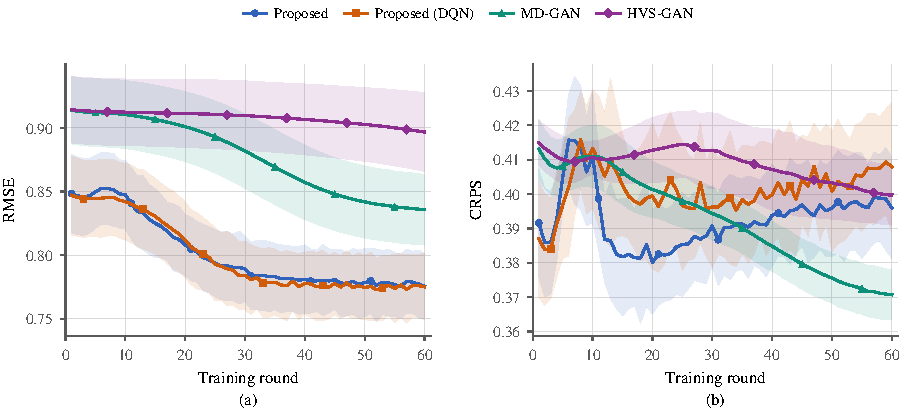
\includegraphics[width=\textwidth]{fig1_convergence.pdf}
\caption{Convergence against federated GAN baselines: (a) RMSE and (b) CRPS
versus training round. Bands are 95\% confidence intervals over five seeds.
Note that MD-GAN overtakes the proposed method on CRPS near round~45.}
\label{fig:conv}
\end{figure*}

\begin{figure*}[!t]
\centering
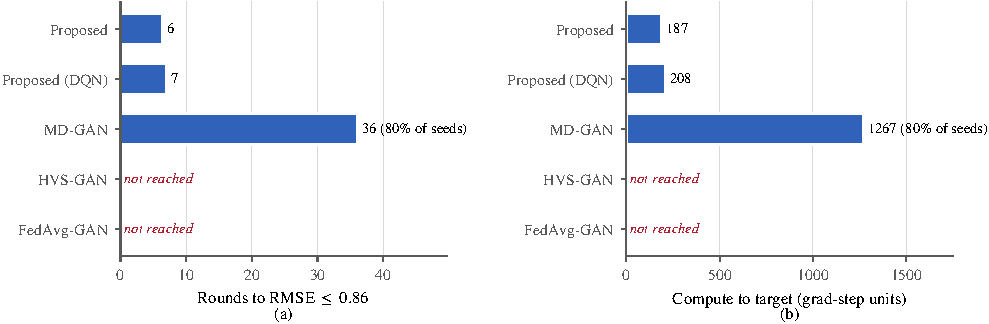
\includegraphics[width=\textwidth]{fig2_cost_to_target.pdf}
\caption{Cost of first reaching RMSE $\leq 0.86$: (a) training rounds and
(b) gradient-step work. Annotations give the fraction of seeds reaching the
target; HVS-GAN and FedAvg-GAN do not reach it in any seed within 60 rounds.}
\label{fig:cost}
\end{figure*}

\begin{figure*}[!t]
\centering
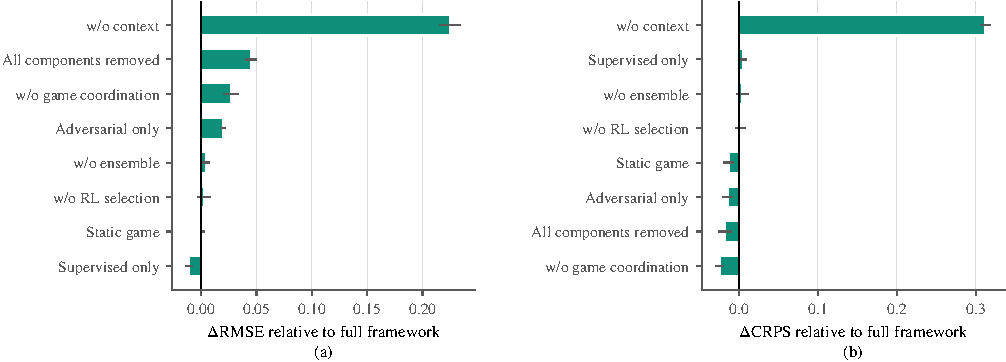
\includegraphics[width=\textwidth]{fig3_ablation.pdf}
\caption{Component ablation: change in (a) RMSE and (b) CRPS when each
component is removed, relative to the full framework. Positive values indicate
that removal degrades performance. Error bars are 95\% confidence intervals
over five seeds.}
\label{fig:ablation}
\end{figure*}

\begin{figure*}[!t]
\centering
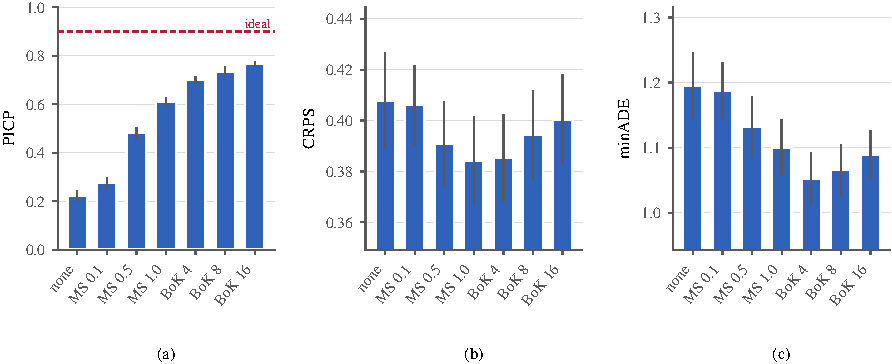
\includegraphics[width=\textwidth]{fig4_calibration.pdf}
\caption{Effect of the diversity mechanism on (a) interval calibration,
(b) CRPS and (c) minADE. Panels (b) and (c) use a non-zero baseline; the plotted
range is a few percent of the value. MS: mode-seeking regularisation;
BoK: best-of-$k$ supervision.}
\label{fig:calib}
\end{figure*}

\begin{figure}[!t]
\centering
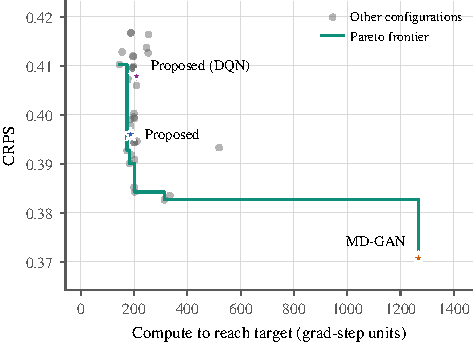
\includegraphics[width=\columnwidth]{fig5_pareto.pdf}
\caption{Accuracy versus cost across all evaluated configurations, with the
Pareto frontier. The proposed configuration sits at the low-cost end; MD-GAN
attains lower CRPS at substantially higher computation.}
\label{fig:pareto}
\end{figure}

\begin{figure*}[!t]
\centering
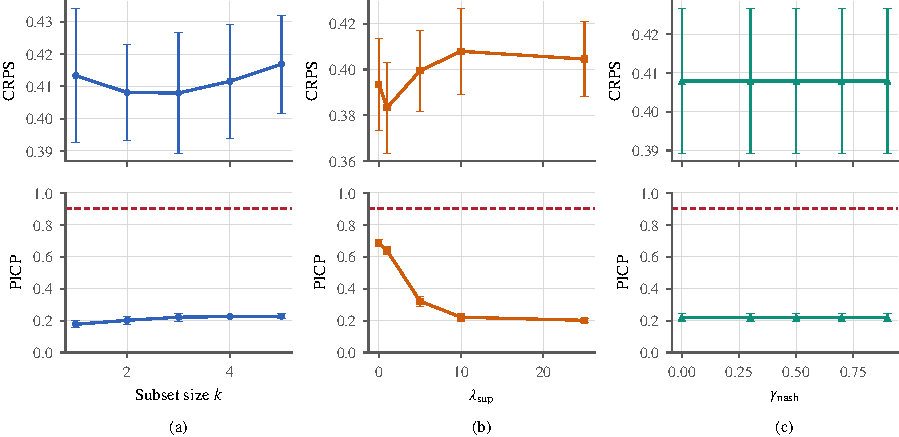
\includegraphics[width=\textwidth]{fig6_sensitivity.pdf}
\caption{Sensitivity of CRPS (top) and PICP (bottom) to (a) the active subset
size $k$, (b) the supervision weight $\lambda_{\rm sup}$ and (c) the
interference coefficient $\gamma_{\rm nash}$, which has no measurable effect.}
\label{fig:sens}
\end{figure*}

\begin{figure*}[!t]
\centering
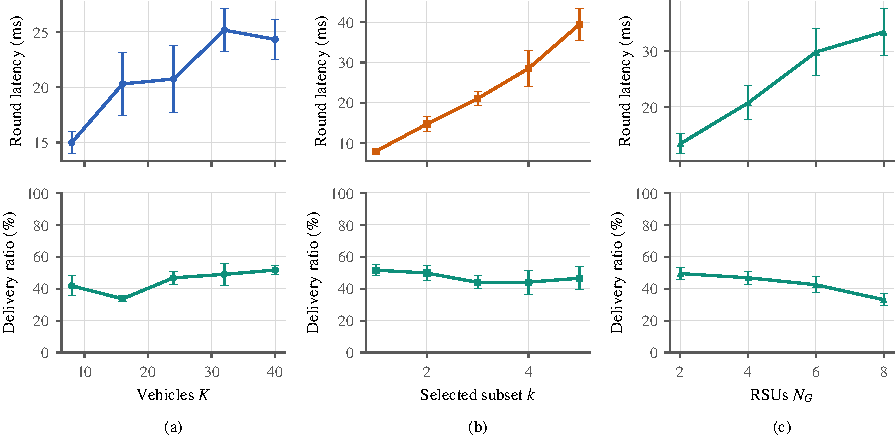
\includegraphics[width=\textwidth]{fig7_ns3_scalability.pdf}
\caption{Measured IEEE 802.11p behaviour of one synchronisation round: round
latency (top) and delivery ratio (bottom) versus (a) vehicle count,
(b) selected subset size and (c) RSU count, for a 600\,m deployment.}
\label{fig:ns3}
\end{figure*}

\begin{table*}[!t]
\centering
\caption{Component ablation. Mean\,$\pm$\,s.d. over five seeds. Significance is a paired Wilcoxon signed-rank test of CRPS against the full framework, Holm-corrected across variants ($^{\ast}p<0.05$, $^{\ast\ast}p<0.01$, $^{\ast\ast\ast}p<0.001$). Compute is gradient-step units spent reaching RMSE\,$\leq$\,0.86.}
\label{tab:ablation}
\begin{tabular}{lccccc}
\toprule
Variant & RMSE $\downarrow$ & CRPS $\downarrow$ & minADE $\downarrow$ & PICP $\rightarrow$0.90 & Compute $\downarrow$ \\
\midrule
\textbf{Full framework} & 0.775\,$\pm$\,0.030 & 0.408\,$\pm$\,0.021 & 1.194\,$\pm$\,0.059 & 0.222\,$\pm$\,0.028 & 208 \\
w/o RL-based selection & 0.778\,$\pm$\,0.032 & 0.410\,$\pm$\,0.018 & 1.199\,$\pm$\,0.049 & 0.220\,$\pm$\,0.013 & 196 \\
w/o ensemble feedback & 0.780\,$\pm$\,0.026 & 0.413\,$\pm$\,0.015 & 1.200\,$\pm$\,0.038 & 0.227\,$\pm$\,0.014 & 253 \\
w/o game coordination & 0.802\,$\pm$\,0.033 & 0.384\,$\pm$\,0.020 & 1.149\,$\pm$\,0.056 & 0.336\,$\pm$\,0.037 & 334 \\
w/o online adaptation (static game) & 0.776\,$\pm$\,0.030 & 0.395\,$\pm$\,0.021 & 1.158\,$\pm$\,0.054 & 0.238\,$\pm$\,0.034 & 210 \\
w/o supervised term & 0.795\,$\pm$\,0.032 & 0.393\,$\pm$\,0.023 & 1.085\,$\pm$\,0.052 & 0.684\,$\pm$\,0.020 & 519 \\
w/o adversarial term & 0.764\,$\pm$\,0.029 & 0.413\,$\pm$\,0.018 & 1.192\,$\pm$\,0.051 & 0.166\,$\pm$\,0.016 & 155 \\
w/o context conditioning & 1.000\,$\pm$\,0.022 & 0.720\,$\pm$\,0.021 & 1.949\,$\pm$\,0.045 & 0.137\,$\pm$\,0.024 & -- \\
all components removed & 0.820\,$\pm$\,0.031 & 0.390\,$\pm$\,0.019 & 1.175\,$\pm$\,0.051 & 0.352\,$\pm$\,0.047 & 184 \\
\bottomrule
\end{tabular}
\end{table*}

\begin{table}[!t]
\centering
\caption{Discriminator-selection strategies under an otherwise identical framework. Mean\,$\pm$\,s.d. over five seeds.}
\label{tab:selection}
\begin{tabular}{lccc}
\toprule
Strategy & RMSE $\downarrow$ & CRPS $\downarrow$ & Compute $\downarrow$ \\
\midrule
DQN (deep RL) & 0.775\,$\pm$\,0.030 & 0.408\,$\pm$\,0.021 & 208 \\
\textbf{Greedy-by-loss} & 0.774\,$\pm$\,0.030 & 0.417\,$\pm$\,0.022 & 188 \\
Random-$k$ & 0.778\,$\pm$\,0.032 & 0.410\,$\pm$\,0.018 & 196 \\
Round-robin & 0.774\,$\pm$\,0.030 & 0.407\,$\pm$\,0.019 & 188 \\
All discriminators & 0.773\,$\pm$\,0.030 & 0.414\,$\pm$\,0.018 & 247 \\
\bottomrule
\end{tabular}
\end{table}

\begin{table}[!t]
\centering
\caption{Effect of the diversity mechanism on predictive calibration. Without it the generator ignores its latent input and its nominal 90\% interval covers only 26\% of targets.}
\label{tab:diversity}
\begin{tabular}{lccc}
\toprule
Mechanism & PICP $\rightarrow$0.90 & CRPS $\downarrow$ & minADE $\downarrow$ \\
\midrule
None (conditional-mean supervision) & 0.222\,$\pm$\,0.028 & 0.408\,$\pm$\,0.021 & 1.194\,$\pm$\,0.059 \\
Mode-seeking, $\lambda_{\rm div}=0.1$ & 0.275\,$\pm$\,0.028 & 0.406\,$\pm$\,0.018 & 1.188\,$\pm$\,0.049 \\
Mode-seeking, $\lambda_{\rm div}=0.5$ & 0.482\,$\pm$\,0.026 & 0.391\,$\pm$\,0.019 & 1.133\,$\pm$\,0.052 \\
Mode-seeking, $\lambda_{\rm div}=1.0$ & 0.610\,$\pm$\,0.021 & 0.384\,$\pm$\,0.020 & 1.100\,$\pm$\,0.048 \\
Best-of-$k$, $k=4$ & 0.699\,$\pm$\,0.016 & 0.385\,$\pm$\,0.019 & 1.052\,$\pm$\,0.045 \\
Best-of-$k$, $k=8$ & 0.734\,$\pm$\,0.023 & 0.394\,$\pm$\,0.020 & 1.065\,$\pm$\,0.045 \\
Best-of-$k$, $k=16$ & 0.765\,$\pm$\,0.012 & 0.400\,$\pm$\,0.020 & 1.089\,$\pm$\,0.042 \\
\bottomrule
\end{tabular}
\end{table}


% =====================================================================
\begin{thebibliography}{99}
%% TODO: merge with the submitted manuscript's bibliography; only the entries
%% newly required by this revision are listed here.
\bibitem{arjovsky2017wgan}
M.~Arjovsky, S.~Chintala, and L.~Bottou, ``Wasserstein GAN,''
\emph{arXiv:1701.07875}, 2017.

\bibitem{creswell2018gan}
A.~Creswell \emph{et al.}, ``Generative adversarial networks: An overview,''
\emph{IEEE Signal Process. Mag.}, vol.~35, no.~1, pp.~53--65, 2018.

\bibitem{hardy2019mdgan}
C.~Hardy, E.~Le~Merrer, and B.~Sericola, ``MD-GAN: Multi-discriminator
generative adversarial networks for distributed datasets,'' in \emph{Proc. IEEE
IPDPS}, 2019, pp.~866--877.

\bibitem{wu2024hvsgan}
L.~Wu, H.~Lin, and X.~Wang, ``Federated training generative adversarial networks
for heterogeneous vehicle scheduling in IoV,'' \emph{IEEE Internet Things J.},
2024.

\bibitem{devika2024vadgan}
S.~Devika \emph{et al.}, ``VADGAN: An unsupervised GAN framework for enhanced
anomaly detection in connected and autonomous vehicles,'' \emph{IEEE Trans. Veh.
Technol.}, vol.~73, no.~9, pp.~12\,458--12\,467, 2024.

\bibitem{luo2025wgan}
X.~Luo \emph{et al.}, ``High-risk powered two-wheelers scenarios generation for
autonomous vehicle testing using WGAN,'' \emph{Traffic Injury Prevention},
vol.~26, no.~2, pp.~243--251, 2025.
\end{thebibliography}

\end{document}
